\documentclass{article}
\usepackage[T1]{fontenc}
\usepackage[utf8]{inputenc}
\usepackage{anysize}
\marginsize{2.5cm}{2.5cm}{1cm}{2.5cm}
\usepackage{amsmath} %koniecznie
\usepackage{amssymb,amsfonts,amsthm}%dodatkowo
\usepackage{tikz}
\usepackage{pgfplots}
\usepackage{gensymb}
\usepackage{polski}
\usepackage{physics}


\title{Fizyka dla Informatyków, wykład\\ Sprawozdanie z realizacji drugiego zadania zespołowego programistycznego}
\author{Jan Bylicki \and Jan Chlebek \and Ryszard Dotka \and Marcin Kasznia}
\date{31 sierpnia 2020}

\begin{document}

\maketitle

\section{Wstęp}
Zadanie programistyczne zrealizowano, zgodnie z sugestiami, przy pomocy języka Python na platformie kwantowej IBM w notatniku Jupytera. Otrzymane wyniki wypisano w ostatniej komórce i na ich podstawie obliczono stan kubitu przy pomocy programu \verb+Mathematica+.\\
Jako dane wejściowe (na podstawie numerów indeksów) obliczono co następuje:
\begin{align*}
    k_1&=1\\
    k_2&=1\\
    k_3&=1
\end{align*}
W dalszej części sprawozdania przedstawiono informacje formalne oraz prezentacje przeprowadzonych pomiarów.

\section{Skład zespołu}
Zadanie zostało zrealizowane w zespole o następującym składzie:
\begin{enumerate}
    \item Jan Bylicki (I4.1; 145441; jan.bylicki@student.put.poznan.pl)
    \item Jan Chlebek (I4.1; 145380; jan.chlebek@student.put.poznan.pl)
    \item Ryszard Dotka (I4.1, 145305; ryszard.dotka@student.put.poznan.pl)
    \item Marcin Kasznia (I5.1; 145379; marcin.kasznia@student.put.poznan.pl)
\end{enumerate}

\section{Wykaz prac wykonanych przez członków zespołu}
    Zadanie zostało rozwiązane wspólnie podczas dwóch spotkań z wykorzystaniem komunikatora głosowego. W przeciwieństwie do pierwszego zespołowego zadania programistycznego całość stanowi pracę wspólną bez wyraźnego podziału obowiązków.
    

\section{Procentowy udział członków zespołu w realizacji projektu}
\begin{enumerate}
    \item Jan Bylicki: 25\%
    \item Jan Chlebek: 25\%
    \item Ryszard Dotka: 25\%
    \item Marcin Kasznia: 25\%
\end{enumerate}
\section{Wykaz przesłanych plików}
    Kod źródłowy programu: \verb+Source_2_145380.zip+, zawierający:
    \begin{enumerate}
        \item Kod źródłowy dla symulatora kwantowego: \verb+QSim.ipynb+ i \verb+QSim.pdf+
        \item Kod źródłowy obliczeń w Mathematice: \verb+Obliczenia.nb+ i \verb+Obliczenia.pdf+
        
    \end{enumerate}
\section{Wykaz zapożyczonych bibliotek}
W projekcie wykorzystano następujące zewnętrzne biblioteki:
    \begin{enumerate}
        \item \verb+qiskit+
        \item \verb+math+
    \end{enumerate}
\section{Zrzuty ekranowe ilustrujące działanie programu}
Obwody kwantowe przygotowane dla pomiarów x, y, z:\\
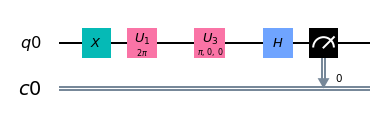
\includegraphics[]{pomiarx.png}\\
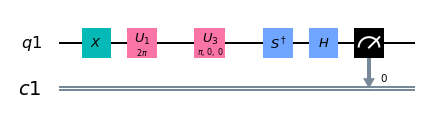
\includegraphics[]{pomiary.png}\\
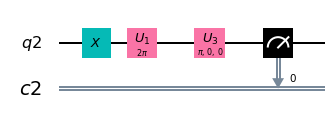
\includegraphics[]{pomiarz.png}\\
W tym miejscu warto wskazać, iż kolejność zastosowania bramek $U_1$ i $U_3$ nie jest w tym przypadku istotna, gdyż iloczyn macierzy im odpowiadający (dla przyjętych wartości wejściowych) jest przemienny.\\
Pomiary przeprowadzono dla próby $n=4000$. Poniżej zaprezentowano rozkład prawdopodobieństw (prawdopodobieństwa uzyskania danego wyniku) dla każdego typu pomiaru.
\begin{center}
    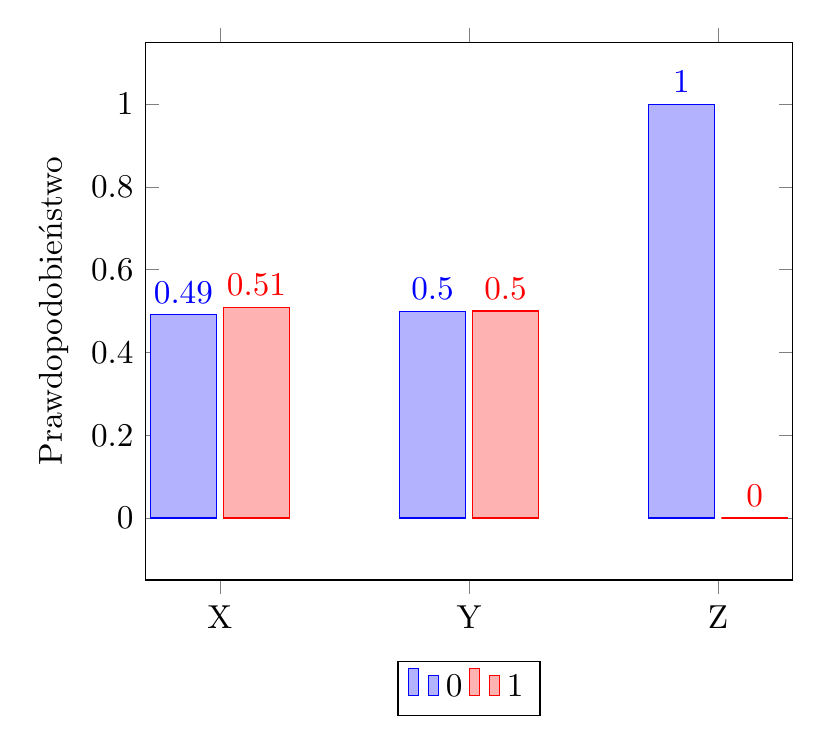
\begin{tikzpicture}[scale=1.2]
        \begin{axis}[
            ybar,
            bar width=20pt,
            enlargelimits=0.15,
            legend style={at={(0.5,-0.15)},
              anchor=north,legend columns=-1},
            ylabel={Prawdopodobieństwo},
            symbolic x coords={X,Y,Z},
            xtick=data,
            nodes near coords,
            nodes near coords align={vertical},
            ]
        \addplot coordinates {(X,0.49125) (Y,0.49925) (Z,1)};
        \addplot coordinates {(X,0.50875) (Y,0.50075) (Z,0)};
        \legend{0,1}
        \end{axis}
    \end{tikzpicture}
\end{center}

Szczegółowe pomiary prawdopodobieństwa:\\
\begin{center}
\begin{tabular}{l|l|l|}
\cline{2-3}
                        & 0       & 1       \\ \hline
\multicolumn{1}{|l|}{X} & 0.49125 & 0.50875 \\ \hline
\multicolumn{1}{|l|}{Y} & 0.49925 & 0.50075 \\ \hline
\multicolumn{1}{|l|}{Z} & 1.0     & 0.0     \\ \hline
\end{tabular}
\end{center}
\section{Wyniki}
Do obliczenia stanu kubitu w eksperymencie posłużono się programem \verb+Mathematica+. Całość obliczeń przedstawiono w załączonym notatniku (plik \verb+Obliczenia+).\\
Stan kubitu uzyskany w eksperymencie przedstawia się następująco:
$$ q=\left(\begin{matrix}0.999961 \\-0.00874899-0.000749913 i\end{matrix}\right)$$
Natomiast stan kubitu wyliczony teoretycznie:
$$q_0=\left(\begin{matrix}-1\\0\end{matrix}\right)$$
Znak wyniku może zostać zignorowany, gdyż wynika on z przyjmowania odmiennej globalnej fazy kubitu na drodze eksperymentalnej. Oznacza to, że faktyczna wartość przyjmowana do obliczeń analitycznych wynosi:
$$q_0=\left(\begin{matrix}1\\0\end{matrix}\right)$$
Błąd względny określony został jako: $$\delta_x=\frac{\Delta x}{x_0}=\frac{x-x_0}{x_0}$$ gdzie: $x$ to wartość mierzona a $x_0$ wartość dokładna.\\
Błąd względny wartości otrzymanej eksperymentalnie (odniesiony wyłącznie do pierwszej wartości wektora) wynosi:
$$\delta_q=\frac{q-q_0}{q_0}=\frac{0.999961-1}{1}=-0.000039=-0.0039\%$$
Błąd w mierzeniu wartości na drodze eksperymentalnej jest zdecydowanie mniejszy niż $2\%$.\\
Warto zauważyć, że tak niski błąd mógł wynikać z faktu, iż uzyskany stan kubitu dopowiada stanowi $\ket{0}$, czyli domyślnemu stanowi startowemu.




\end{document}
